% Define document class
\documentclass[twocolumn]{aastex63}
\DeclareRobustCommand{\Eqref}[1]{Eq.~\ref{#1}}
\DeclareRobustCommand{\Figref}[1]{Fig.~\ref{#1}}
\DeclareRobustCommand{\Tabref}[1]{Tab.~\ref{#1}}
\DeclareRobustCommand{\Secref}[1]{Sec.~\ref{#1}}
\newcommand{\todo}[1]{{\large $\blacksquare$~\textbf{\color{red}[#1]}}~$\blacksquare$}
\newcommand{\mr}[1]{{\textbf{\color{green!75!black}[#1]}}}
% \usepackage{cuted}
\usepackage{flushend}
\usepackage{amsmath}
\graphicspath{{./figures/}}

\begin{document}

% Title
\title{\todo{title}}

\author[0009-0008-2061-4946]{C.~A.~Burt}
\affiliation{University of Arizona, Department of Astronomy \& Steward Observatory, 933 N.~Cherry Ave., Tucson, AZ 85721, USA}

\author[0000-0002-6718-9472]{M.~Renzo}
\affiliation{University of Arizona, Department of Astronomy \& Steward Observatory, 933 N.~Cherry Ave., Tucson, AZ 85721, USA}

\author[0000-0002-2215-1841]{A.~Grichener}
\affiliation{University of Arizona, Department of Astronomy \& Steward Observatory, 933 N.~Cherry Ave., Tucson, AZ 85721, USA}

\author{\todo{TBD}}

\begin{abstract}
  For very massive stars ($M \gtrsim 30 \, M_{\odot}$), there are two major modes of mass transfer; namely case A and case B. In most circumstances, the bulk of a star's radial expansion occurs during the Hertzsprung gap, providing more opportunities for case B mass transfer to occur. However, very massive stars undergo significant radial expansion during the main sequence which increase the relative probability that case A mass transfer occurs. In this research note, we find that stellar models with broad convective boundary mixing indicates that case A mass transfer dominates in the mass regime $M \gtrsum 75 \, M_{\odot}$. This effect does not occur in cases of no convective boundary mixing or very conservative boundary mixing. These results suggest that case A mass transfer occurs in more situations than previously believed and affect the conditions creating X-ray binaries and gravitational wave progenitors.
\end{abstract}

\section{Mass Transfer Between Very Massive stars }

Binary stars with a sufficiently small orbital separation undergo a
mass transfer phase in which one donor star transfers mass to an
accretor star. As the stellar main sequence progresses, the donor
star's radius expands until it exceeds its Roche Lobe, allowing for
the surface to become gravitationally bound to the accretor, which
triggers a mass transfer phase. For very massive stars
($>30M_{\odot}$), this occurs in two cases.  Case A mass transfer
occurs while the donor star is in the main sequence, while case B mass
transfer occurs while the donor star is burning helium in its core
\mr{\cite{kippenhahn:67}}. In both cases, the accretor gains the mass
lost by the donor until the masses are equal \mr{no, typically until
  m2=1.1*(m2 before RLOF), see \cite{packet:81}}, or the mass gainer
cannot accrete due to increased rotational velocity caused by angular
momentum conservation. The increase in total mass of the accretor,
typically a main sequence star during RLOF, causes by the virial
theorem an increase in its central temperature and thus in the extent
of core-convection resulting in access to more nuclear fuel and
elongation of the lifespan of the star (\citealt{neo:77} but see also
\citealt{braun:95}) and potentially modifying its internal structure
and future evolution \citep[e.g.,]{renzo:23, , wagg:24, landri:24,
  nathaniel:24}.


\begin{figure*}[htbp]
  \centering
  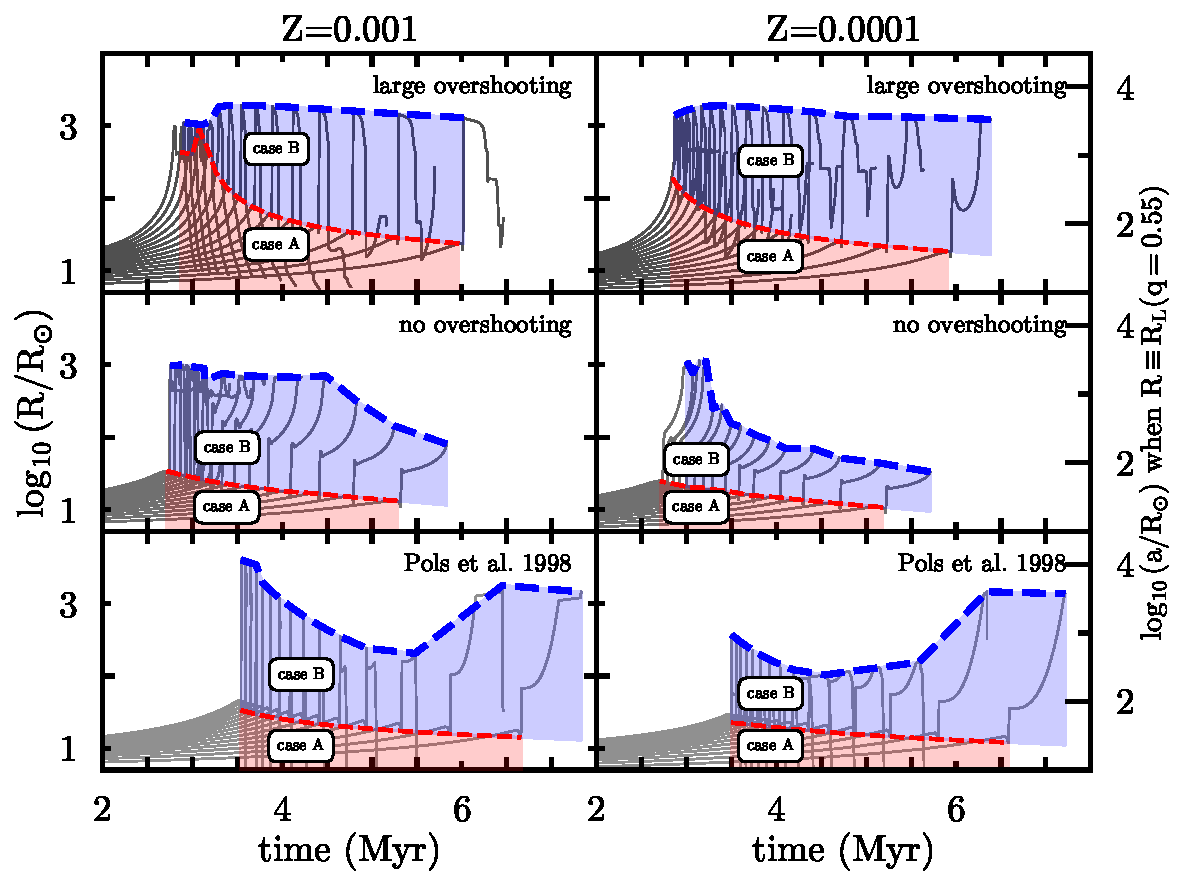
\includegraphics[width=0.9\textwidth]{radii}
  \caption{Each panel contain 15 stellar models spanning from a $30 \, M_{\odot}$ star on the right to a $100 \, M_{\odot}$ with intervals of width $5 \, M_{\odot}$. The top panels plot models that feature broad convective boundary mixing, the middle panels plot models that do not feature overshooting, and the bottom panels plot models generated from COMPAS using data from \cite{pols:98}. The left panels have a metallicity $Z=0.001$ and the right panels have a metallicity $Z=0.0001$}
  \label{fig:R_t_donor}
\end{figure*}


In nature, case B mass transfer is observed more often than case A
mass transer --CITE--. This result is expected from theory; stars in
most mass ranges expand most prominently post-main sequence in the
Hertzsprung gap \citep{vandenheuvel:69}. However, very massive stars
undergo a drastic expansion in radius during their main
sequence. \citep[e.g.,][]{brott:11}. This increases the relative
abundance of instances of case A mass transfer \citep{demink:08}, which has significant implications on the evolution of X-ray binary systems and gravitational wave progenitors.

\mr{probably already from the ``introduction'' we need to say why we
  care, why would readers care? binary interactions are crucial to the
formation of GW sources, and in particular for BBH stable mass
transfer may dominate \cite{marchant:21, vanson:21}}

The relative proportion of case A mass transfer in comparison to case
B mass transfer scales with mass of the donor star. This is expected,
as larger stars see greater rates of radial expansion during the main
sequence. This has a significant side effect for stars with($\gtrsim 75M_{\odot}$), case A mass transfer is expected to explain
in all possible mass transfer processes. For stars of lesser mass, the
thermal expansion of the star at the end of the main sequence expands
the star beyond its maximum radius during the main sequence. However,
for stars in this mass range, the radius expands drastically during
the main sequence, such that the maximum radius during the main
sequence and helium core burning phase are similar.

\mr{maybe here you need to explain a bit what we do in this research
  note before jumping in the results!}  \todo{Describe the models you
  run (which input physics, which code) with and without overshooting,
  and the pols+98 models (just reference)}

In order to demonstrate the change in ratio between instances of case
A and case B mass transfer, we modelled 60 stars while varying mass
($30-100 M_{\odot}$; of $5M_{\odot}$ intervals), metallicity
($Z = 0.001,0.001$) and model of boundary mixing. The top panels of FIGURE are determined from the exponential boundary mixing model from \cite{04} fit to the expected values from the step boundary mixing model from \cite{brott:11}. This is configured in \cite{claret:18}. This ``broad convective boundary mixing'' model is compared to a model that does not consider boundary mixing. Both models were instructed to end before the carbon burning phase could commence.

In addition, 30 models generated using the rapid population synthesis code COMPAS using models generated from data gathered in \cite{pols:98} are plotted in the bottom panels of FIGURE. These models match the metallicities of the stellar evolution models in the other panels. These models include data until core collapse.

Stellar radius is strongly dependent on many parameters. This research note specifically consideres different regimes of convective boundary mixing

Convective boundary mixing has a strong effect on stellar
radius \cite{brott:11, johnston:24}, which determines Roche lobe
overflow. The vast differences in the ratio of expected abundances of case A and case B mass transfer are consequentially expected. The broad convective boundary mixing models limit
case B mass transfer for stars of mass ($\gtrsim 75M_{\odot}$) . In contrast, omitting convective boundary mixing allows case B mass transfer to occur at a significant scale in all mass regimes such that $M<100_{\odot}$. HOW TO CITE Brott's paper suggests broad convective boundary mixing models currently provide the best approximation for observed characteristics of massive stars. As a result, many rapid population synthesis softwares and other stellar mass transfer models may underestimate the abundance of case A mass transfer procedures.

Binary interactions are crucial to the formation of X-ray binaries and gravitational waves sources. in particular for BBH stable mass
transfer may dominate \cite{marchant:21, vanson:21}}


\bibliography{./donorR.bib}
\end{document}

%%% Local Variables:
%%% mode: latex
%%% TeX-master: t
%%% End:
